\chapter{The Polar Front as a major biogeographic boundary in the Southern Ocean} 
\label{ch:polarfront}

\emph{Sections of this chapter have been previously published in \bibentry{Wilkins:2012td}.}

And another try: \cite{Wilkins:2012td}.

\section{Summary}

\section{Introduction}


\section{Methods}
\subsection{Sampling and metagenomic sequencing}

Sampling\footnote{Sampling was performed by Jeffrey M. Hoffman and Jeffrey B. Mcquaid} was conducted on board the RSV \emph{Aurora Australis} during cruise V3 CEAMARC/CASO (Collaborative East Antarctic Marine Census / Climate of Southern Ocean) from 13 December 2007 -- 26 January 2008. 
This cruise occupied the SR3 latitudinal transect from Hobart, Australia (44$^\circ$ S) to the Mertz Glacier, Antarctica (67$^\circ$ S) within a longitudinal range of 140--150$^\circ$ E.
Nineteen samples (16 surface, 3 deep) were obtained along almost the entire latitudinal range \figref{fig:samplemap}.

% the sample map
\begin{figure}[!ht]
  \centering
  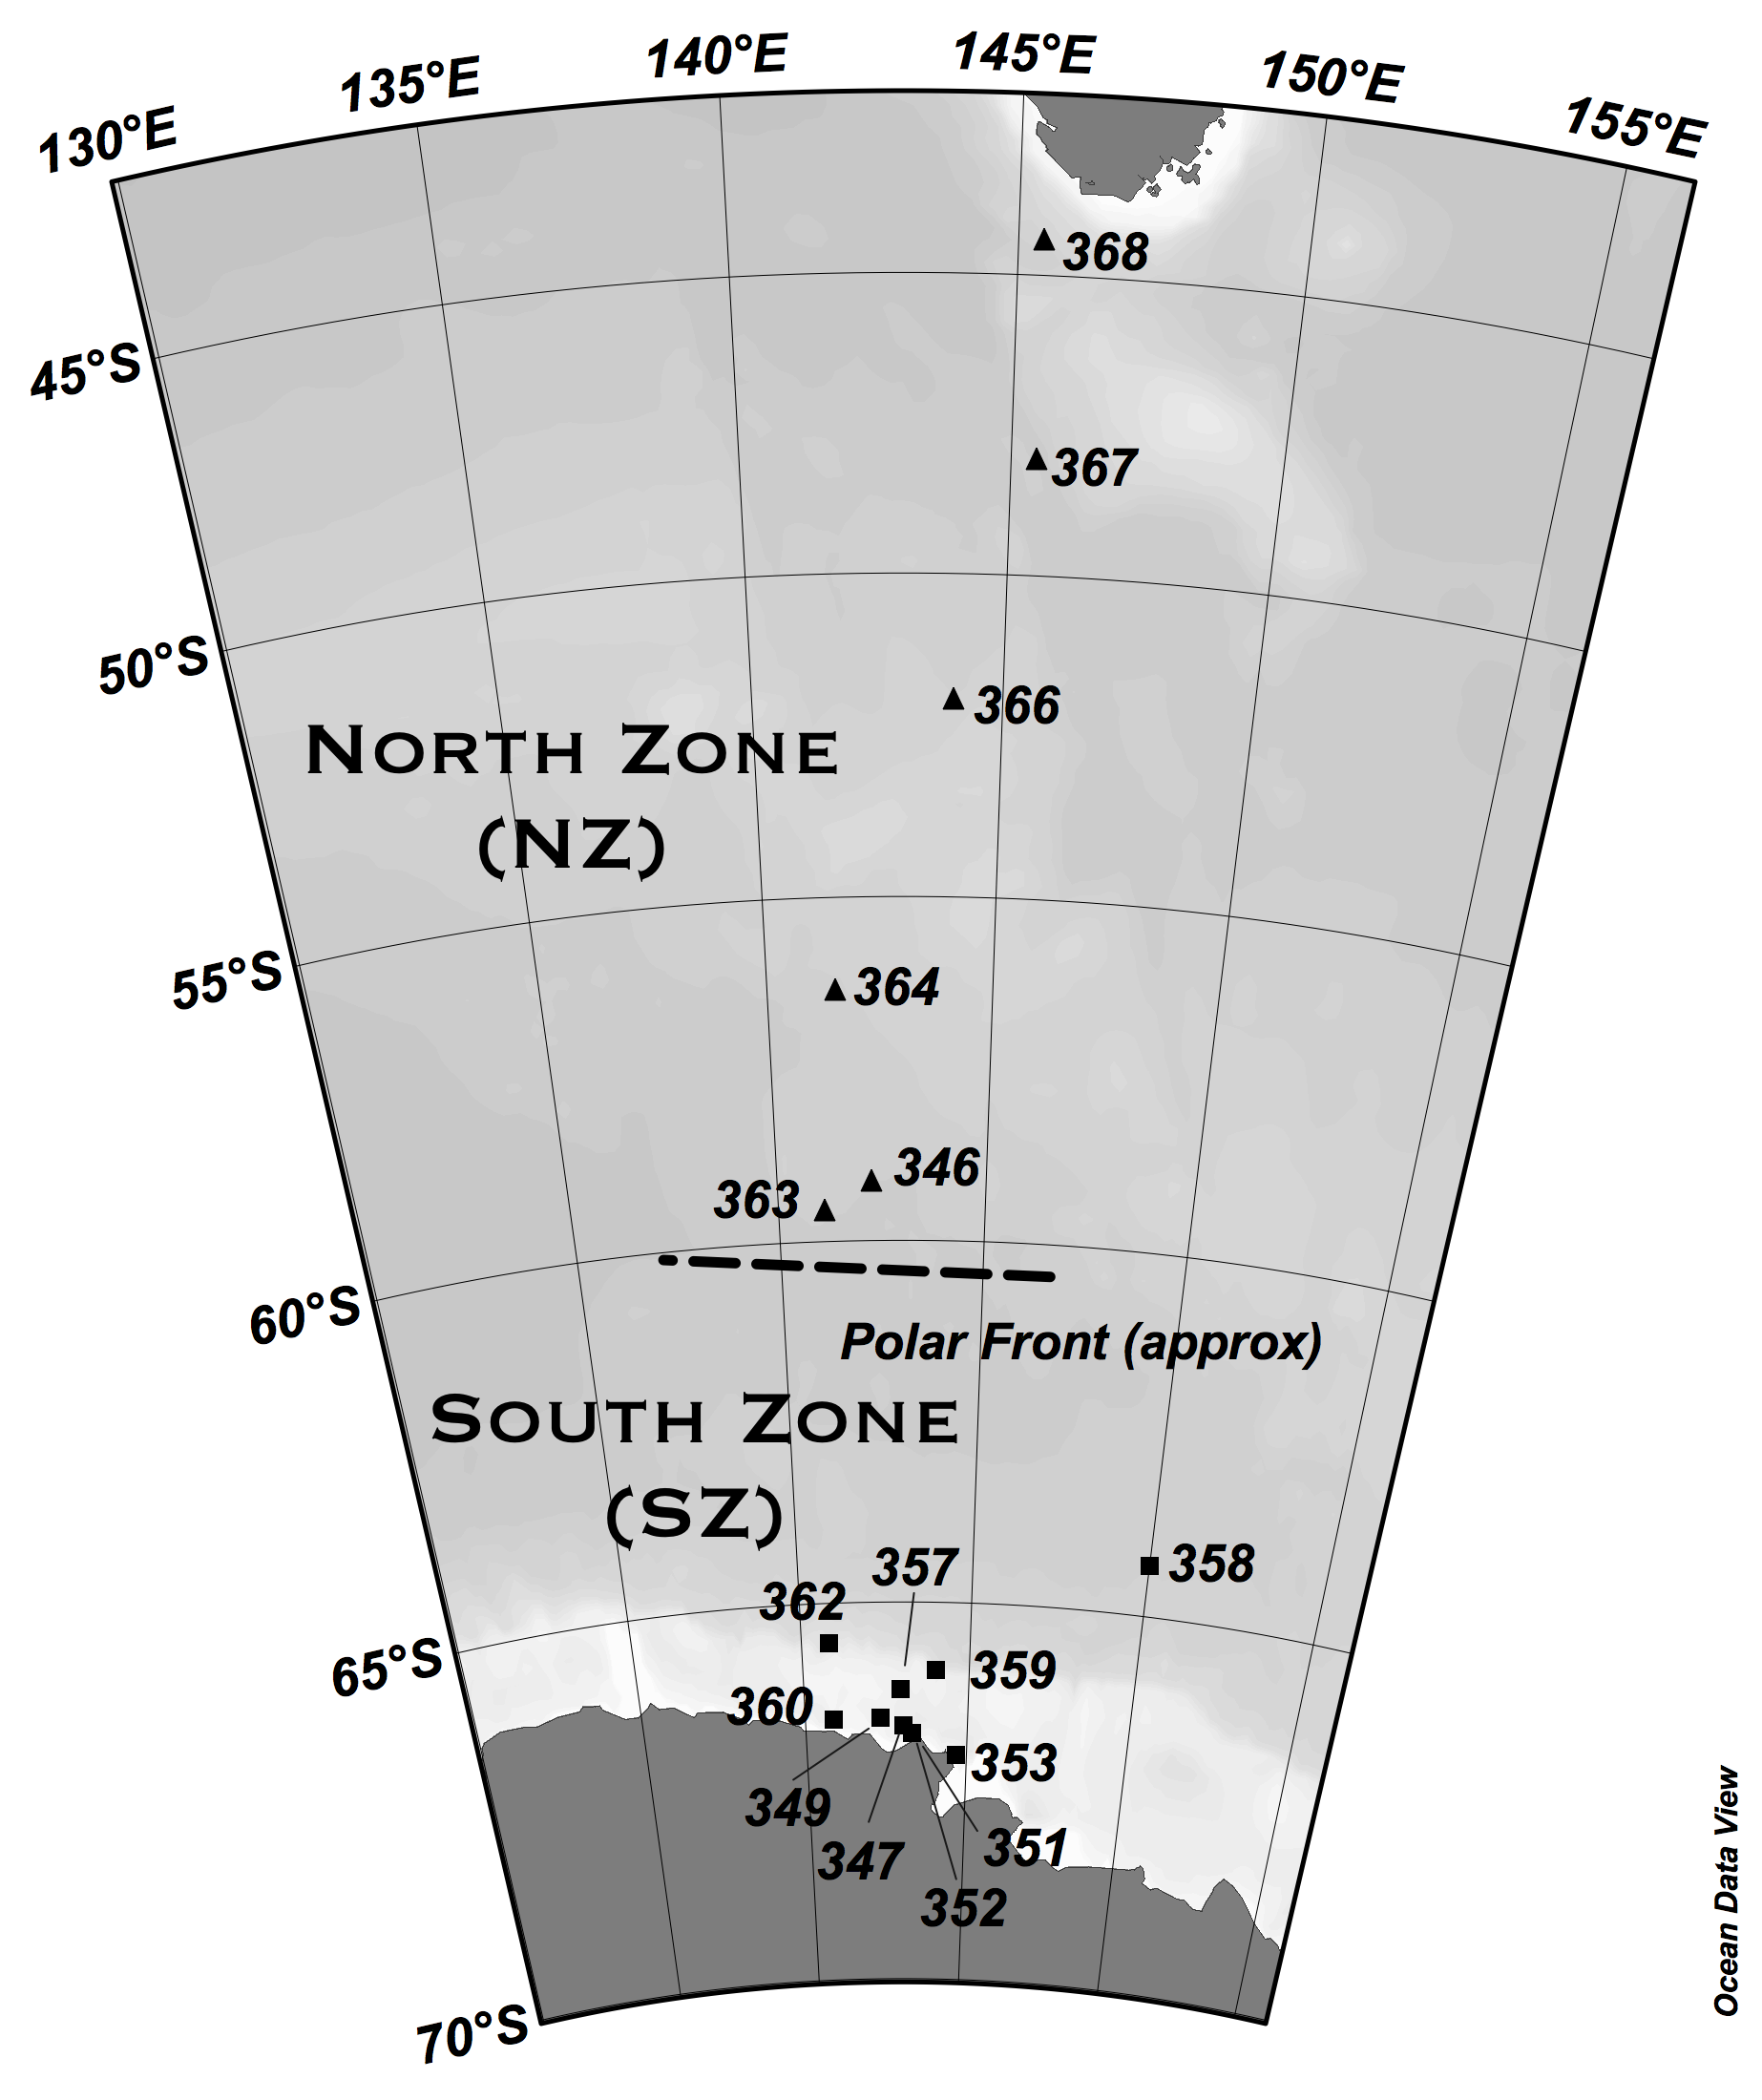
\includegraphics[width=\textwidth]{../polarfront/samplemap.png}
  \caption[Map showing sites of seawater samples used in the Polar Front study]{Sites of seawater samples used in this study. 
  Squares indicate surface samples from the North Zone; crosses samples from the South Zone. 
  The dashed line represents the Polar Front.}
  \label{fig:samplemap}
\end{figure}


A range of data were recorded by integrated instruments on the RSV \emph{Aurora Australis} including location, water column depth, water temperature, salinity, fluorescence and meterological data (TODO provide table).
These data were used to locate the (TODO abbreviations package? PFZ) based on a surface temperature gradient of $\sim$ 1.35 $^\circ$C across a distance of 45--65 km, placing the (TODO abbreviations? PF) at approximately $-59.70^\circ$ of latitude, consistant with previous descriptions TODO EDITING HERE NEED SOKOLOV AND RINTOUL REF

At each station, $\sim$ 500 L of seawater was pumped from $\sim$ 2 m below the sea surface into drums stored at ambient temperature on deck. 
In the case of deep samples, $\sim$ 10--50 L of seawater was collected opportunistically from Niskin bottles attached to a CTD (Conductivity, Temperature and Depth TODO give infor on CTD - SeaBird?) instument operated by an unrelated oceanographic project.
Seawater samples were prefiltered through a 20 $\mu$m plankton net, then filtrate was captured on sequential 3.0 $\mu$m, 0.8 $\mu$m and 0.1 $\mu$m polyethersulfone membrane filters (Supor membrane disc filter; Pall Life Sciences TODO location), and immediately stored at $-20$ $^\circ$C \cite{Rusch:2007ez,Ng:2010cd}.

DNA extraction\footnote{DNA extraction was performed by Cynthia Andrews-Pfannkoch and others at the J. Craig Venter Institute} was performed at the J. Craig Venter Institute (Rockville, USA) as described in \citet{Rusch:2007ez}.
Pyrosequencing was performed on a GS20 FLX Titanium instrument (Roche, Branford, USA) also at the J. Craig Venter Institute as described in \citet{Lauro:2010jna}.
Duplicate reads and reads with many pyrosequencing errors were removed as described in \citet{Lauro:2010jna}.

\subsection{Phylogenetic analysis of metagenomic data}
\subsection{Functional analysis of metagenomic data}

\section{Results}
\subsection{Metagenomic sequencing}
\subsection{Phylogenetic analysis of metagenomic data}
\subsection{Functional analysis of metagenomic data}

\section{Discussion}

\section{Conclusions}

